\documentclass[12pt,a4paper]{report}

\usepackage[left=2cm, right=2cm, top=4cm, bottom=2cm]{geometry}
\usepackage{enumitem}
\usepackage{fontspec}
\usepackage{tikz}
\usepackage{amsmath}
\usepackage{algpseudocode}

%Eventos
\algblockdefx[Initially]{Initially}{EndInitially}{\textbf{initially do}}{\textbf{end initially}}
\algblockdefx[Upon]{Upon}{EndUpon}[1]{\textbf{upon #1}}{\textbf{end upon}}

\begin{document}
	%Portada
\begin{titlepage}
	\centering
	{\scshape\LARGE Universidad Nacional Autónoma de México \par}
	\vspace{1cm}
	{\scshape\Large Computación Distribuida\par}
	\vspace{1.5cm}
	{\huge\bfseries Tarea 7\par}
	\vspace{.5cm}
	{\Large\itshape Edgar Quiroz Castañeda \par}
	\vspace{.5cm}
	{\Large\itshape Jerónimo Almeida Rodríguez \par}
	\vfill
	 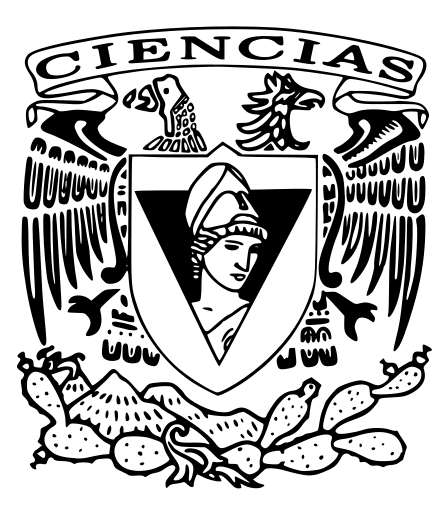
\includegraphics[width=0.5\textwidth]{escudo_f-ciencias.png}
	\vfill

	{\large Jueves 1 de noviembre del 2018 \par}
\end{titlepage}

\pagebreak
\setlength{\voffset}{-0.75in}
\setlength{\headsep}{5pt}

%Ejercicios
\begin{enumerate}
	%1
	\item {
		Considera la ejecución $\alpha$ de la Figura 1. Los retardos máximos
		para cada uno de los eventos son $B_{i, j}$, donde $i$ es el evento
		que envía y $j$ el que recibe.
		\begin{enumerate}
			%a
			\item {
				¿Cuánto vale el retardo máximo de $c$ a $e$ en términos de
				las $B$s? Es decir, dado $real(c)-real(e) \leq x$, ¿cuánto
				vale $x$?\\
				$B_{cd} + B_{de}$
			}

			%b
			\item {
				Anotar los eventos con los relojes escalares y los relojes
				vectoriales.\\
				$a:1, b:2, c:3, d:4, e:5$\\
				$a:(1, 0, 0), b:(1, 1, 0), c:(1, 1, 1), d:(1, 2, 1), e:(2, 2, 1s)$
			}

			%c
			\item {
				¿Cuáles son eventos concurrentes y cuáles no?\\
				Existe una trayectoria que pasa por todos los eventos, por
				lo que ningún par de eventos es concurrente.
			}

			%d
			\item {
				Describe todos los cortes consistentes de $\alpha$.\\
				Si en evento está en $S$, entonces ninguno de los eventos
				que causa puede estar en $T$. Entonces, para generar los
				eventos en $S$, se toma un evento y todos los que este causa,
				poniendo a todos los demás en $T$.\\
				\begin{tabular}{| l | c |}
					\hline
						S & T \\ \hline
						e & a, b, c, d \\ \hline
						d, e & a, b, c \\ \hline
					    c, d, e & a, b \\ \hline
					    a, b, c, d, e & a \\
					\hline
				\end{tabular}
			}
		\end{enumerate}
	}

	%2
	\item {
		Sea $G = (V, E)$ la gráfica dirigida de causalidad de una ejecución
		$\alpha$, $e, e' \in V$ y $L$ un reloj vectorial.\\
		Un evento causó a otro si existe un camino dirigido que inicia en
		el primer evento y acaba en el segundo.\\
		Demuestra que $e$ causó a $e'$ si y sólo si $L(e) < L(e')$.
	}

	%3
	\item {
		Lee los primeros 5 sueños del libro \textit{Einstein's Dream}.
		Redacta un pequeño resumen de cada uno de ellos.
        \begin{itemize}
            \item{\textbf{14 April 1905}\\
                En este primer sueño, se relata una linea de tiempo circular,
                es decir que todo lo que secede, sucedió y está por suceder ya
                lo hizo una cantidad desconocida de veces. Según el cuento, la
                gente, en general no es consciente de esto y vive su vida
                atesorando cada momento cómo si nunca fuera a volver, celebrando
                la unicidad de una primera vez cómo si nunca mas volviera a
                suceder, sufriendo la pérdida de un ser querido cómo si nunca
                más lo fueran a volver a ver.\\
                Pero, de vez en cuando, algunos escogidos recuerdan en
                tormentosos sueños aquellos errores que cometieron y
                malfortunios que vivieron ya tantas veces y que no van a poder
                hacer nada para cambiarlos.\\
            }
            \item{\textbf{16 April 1905}\\
                En este sueño, el tiempo es cómo un riachuelo, fluye en una
                dirección pero a veces arrastra algo inesperado.\\
                Tal es el caso de una viajera anónima del futuro que quedó
                atrapada en este flujo. El problema es que esta viajera sabe
                que levantar una partícula de polvo puede tener efectos tan
                catastróficos cómo la creación de la Union Europea en las
                décadas por venir o la falta de ella. Atormentada por esto,
                encuentra un rincón oscuro dónde no pueda hacer nada que afecte
                el futuro de dónde ha venido.\\
                La gente pasa y, cómo a muchos desafortunados cómo ella, los ven
                y se conmiseran de ellos, sabiendo que no hay manera de
                ayudarlos, pues al hacerlo pueden afectar un futuro que ellos
                mismos no conocen.\\
            }
            \item{\textbf{19 April 1905}\\
                Este escrito nos relata la historia de un hombre y los mundos
                que se bifurcan a partir de una decisión que toma.\\
                En el primer mundo, decide asentarse, trabajar duro, disfrutar
                momentos con sus amigos. Un día conoce a una mujer, la corteja
                a lo largo de unos meses y envejecen juntos.\\
                En el segundo mundo, decide hablar con la mujer de sus sueños.
                Su sonrisa, su risa, su elocuencia al hablar lo enamoran. Lo
                convence de cambiar de ciudad para vivir con ella y viven una
                vida apacionada. Él es feliz.\\
                En el tercer mundo, igual que en el segundo, decide hablar con
                ella, pero ella lo rechaza.\\
                Así se desarrolla la vida en este universo. Cada decisión que se
                toma se bifurca en otros mundos en los que la historia se
                desarrolla de manera diferente; y hay una infinidad de ellos.\\
            }
            \item{\textbf{24 April 1905}\\
                mas
            }
        \end{itemize}
	}

	%4
	\item {
		Sean $A$ y $B$ dos procesos cuyos relojes no están sincronizados,
		pero ambos tienen un $drift$ acotado. Un mensaje de $A$ a $B$
		tarda a lo más $D$, en tiempo real.\\
		Propón un algoritmo para que $B$ estime el tiempo de llegada de un
		mensaje de $A$, si este manda mensajes cada $T$ unidades de tiempo.

		\begin{algorithmic}[1]
			\Initially
			 	\State maxDelay = 0
				\State lastSeen = 0
			\EndInitially
			\Statex

			\Upon{receiving $m$ from $A$}
				\If{getTime() - lastSeen > maxDelay}
					\State maxDelay = getTime() - lastSeen
				\EndIf
				\State lastSeen = getTime()
				\State print('next message at', getTime() + maxDelay)
			\EndUpon
		\end{algorithmic}
	}
\end{enumerate}

\end{document}
